\documentclass{beamer}

\usepackage[utf8x]{inputenc}
\usepackage[english,russian]{babel}
%\usepackage{times}

\usepackage{color, colortbl}
\usepackage{rotating} 
\usepackage{graphicx}
\usepackage{algorithmic}
\usepackage{verbatim}

\usetheme{PetrSU-CS}

%%%%
% Преамбула: основные параметры презентации
% Отредактируйте в соответствии с комментариями
%

\title[%
    % Краткое название работы не используется в этой презентации!
    Разработка приложения распознавания автомобильных номеров
]{%
    % Полное название работы отображается на титульной странице
    Разработка модели распознавания автомобильных
 номеров на основе технологий компьютерного
 зрения
}

% Подзаголовком опишите тип работы:
% - Курсовая работа
% - Выпускная квалификационная работа бакалавра
% - Дипломная работа
% - Магистерская диссертация
\subtitle{Выпускная квалификационная работа бакалавра \\ Направление 09.03.02 --- Информационные системы и технологии}

\author[%
    % Имя и фамилия автора работы отображаются на каждом слайде в нижнем колонтитуле
    Олег Плугин
]{%
    % Имя, отчество и фамилия автора работы отображаются на титульном слайде
    Олег Антонович Плугин
}

\date[%
    % Дата защиты
    16.06.2025
]{%
    % Руководитель
    Научный руководитель: к.ф.-м.н., доцент Д. Ж. Корзун
}

\institute[%
    % Краткое название организации не используется в этой презентации
    ПетрГУ
]{%
    % Полное название организации и подразделения
    Петрозаводский государственный университет\\
	Факультет математики и информационных технологий\\
    Кафедра информатики и математического обеспечения
}


%%%%
%
% Начало содержимого слайдов
%

\begin{document}

\begin{frame}
  \titlepage
\end{frame}

\begin{comment}
\label{content}
\begin{frame}
  \frametitle{Table of Contents}
  \vspace{1.5em}
  \tableofcontents
  \vspace{1.5em}
\end{frame}
\end{comment}

\begin{frame}
\frametitle{Цели и задачи}
%\begin{center}
\begin{block}{Цель работы}
    Разработка прототипа приложения автоматического распознавания автомобильных номеров с видеоряда.
\end{block}
%\end{center}
\begin{block}{Задачи работы}
\begin{enumerate}
    \item Исследовать технологии для задачи распознавания автомобильных номеров
    \item Выбрать наиболее подходящие инструменты
    \item Реализовать прототип приложения 
\end{enumerate}
\end{block}
\end{frame}

%%%%%%%%%%%%%%%%%%%%%%%%%%%%%%%%%%%%%%%%%

\begin{frame}
\frametitle{Актуальность темы}
\begin{itemize}
    \item Системы распознавания объектов применяются в безопасности, транспорте и автоматизации 
    \item Автоматическое распознавание номеров используется на парковках, охраняемых территориях, дорогах общего пользования
    \item Существующие решения дорогие, требовательные к оборудованию, закрытые проекты.
\end{itemize}
\begin{center}

\includegraphics[width=0.6\textwidth]{alrp_example.jpg}
\end{center}
\end{frame}

%%%%%%%%%%%%%%%%%%%%%%%%%%%%%%%%%%%%%%%%%

\begin{frame}
\frametitle{Сравнение существующих решений}
\begin{table}[H]
\centering
\begin{tabular}{|p{2.5cm}|p{3.5cm}|p{2cm}|p{2cm}|}
\hline
\textbf{Название системы} & \textbf{Технологии} & \textbf{Приблизи-тельная стоимость} & \textbf{Точность} \\
\hline
ПОТОК-Паркинг & ИК-камеры, технологии КЗ & 115.000 руб. & 96\% \\ 
\hline
OpenALR & C++, OpenCV, TesseractOCR & 90.000 руб. & 99.02\% \\ 
\hline
POLISCAN Surveillance & LIDAR, технологии КЗ & Неизвестно & Неизвестно (Высокая) \\ 
\hline
AutoTRASSIR & Внутренний алгоритм, три нейронные сети & 80.000 руб. & 99\% \\ 
\hline
\end{tabular}
\end{table}
* КЗ - компьютерное зрение.
\end{frame}

%%%%%%%%%%%%%%%%%%%%%%%%%%%%%%%%%%%%%%%%%

\begin{frame}
\frametitle{Внешний вид рассмотренных систем}
\begin{columns}[T]
    \begin{column}{0.5\textwidth}
    \end{column}
    \begin{column}{0.5\textwidth}
    \end{column}
\end{columns}

\vspace{-1em}
\begin{columns}[T]
    \vspace{1em}
    \begin{column}{0.5\textwidth}
        \vfill
        \begin{figure}
            \centering
            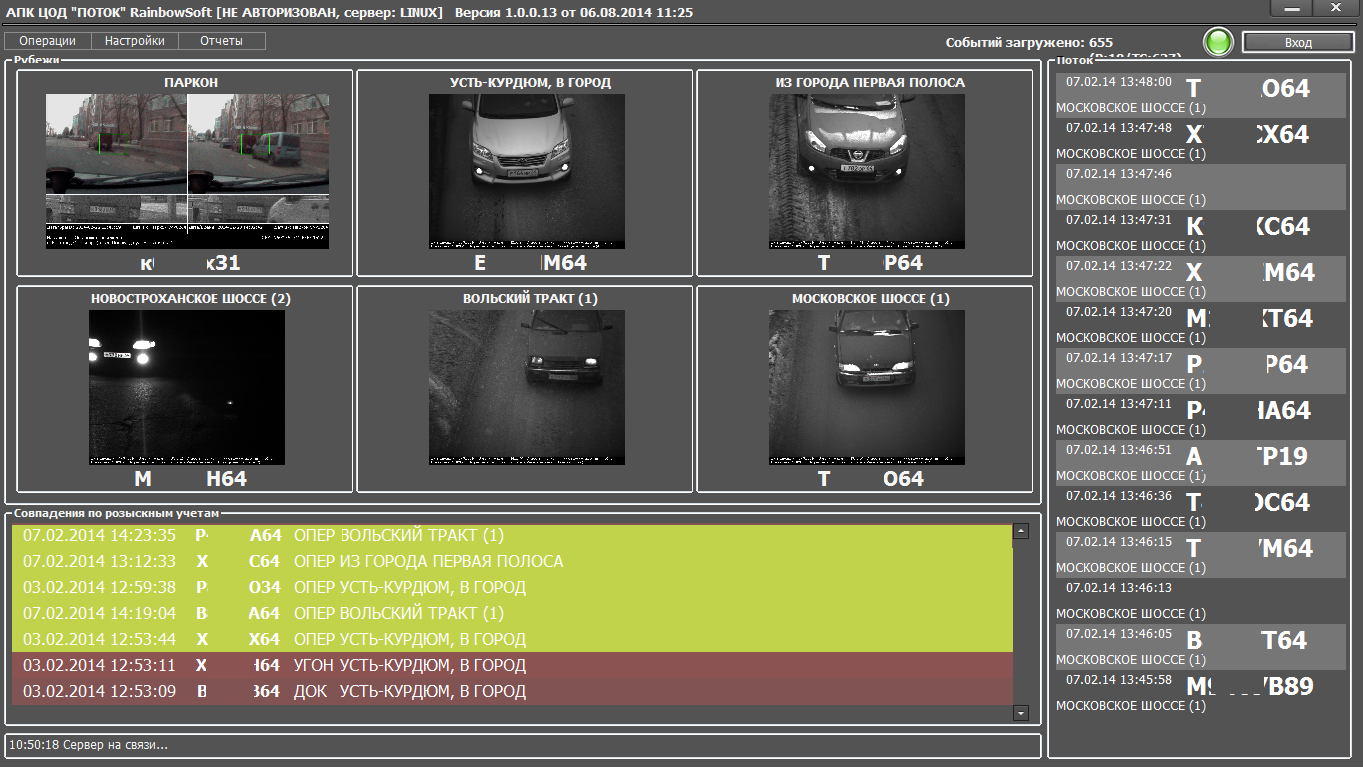
\includegraphics[width=0.8\linewidth]{potok_example.png}
            \vspace{-0.8em}
            \caption{Система ПОТОК}
        \end{figure}
        \vfill
    \end{column}

    \begin{column}{0.5\textwidth}
        \vfill
        \begin{figure}
            \centering
            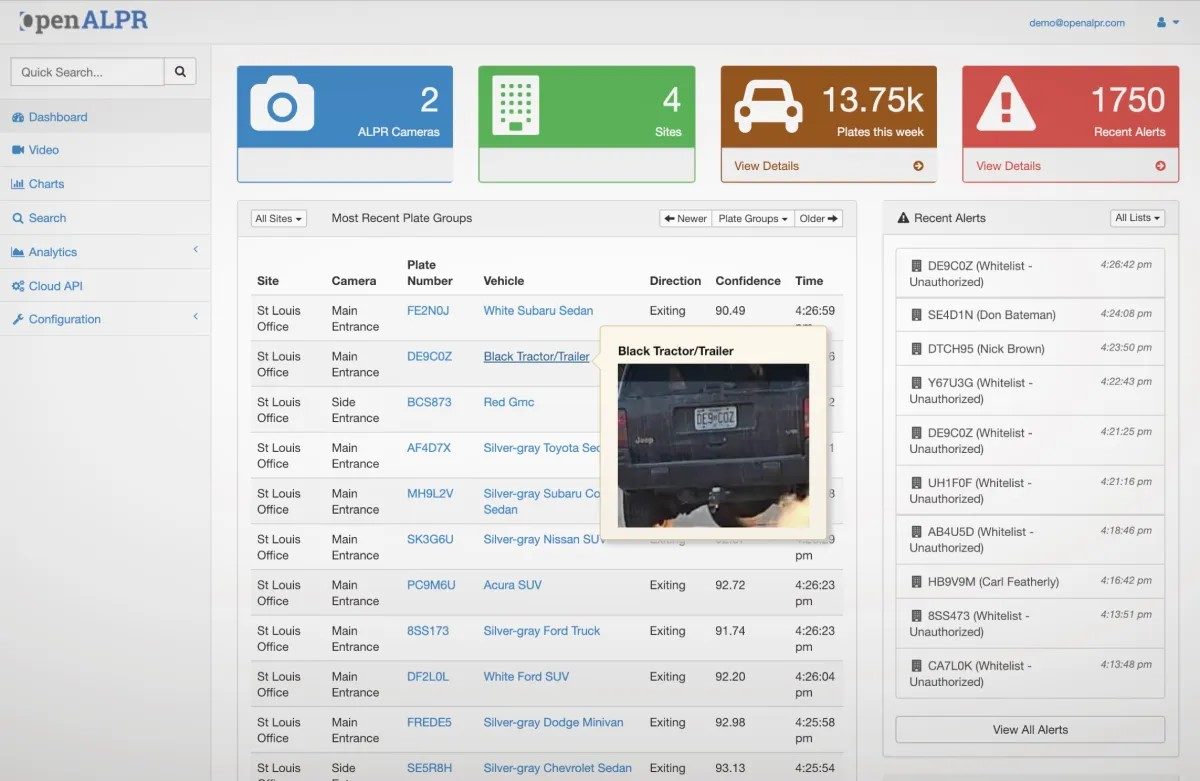
\includegraphics[width=0.8\linewidth]{openalpr_example.jpg}
            \vspace{-0.8em}
            \caption{Система OpenALPR}
        \end{figure}
        \vfill
    \end{column}
\end{columns}

\vspace{-3.5em}
\begin{center}
\end{center}
\begin{center}
    \begin{figure}
        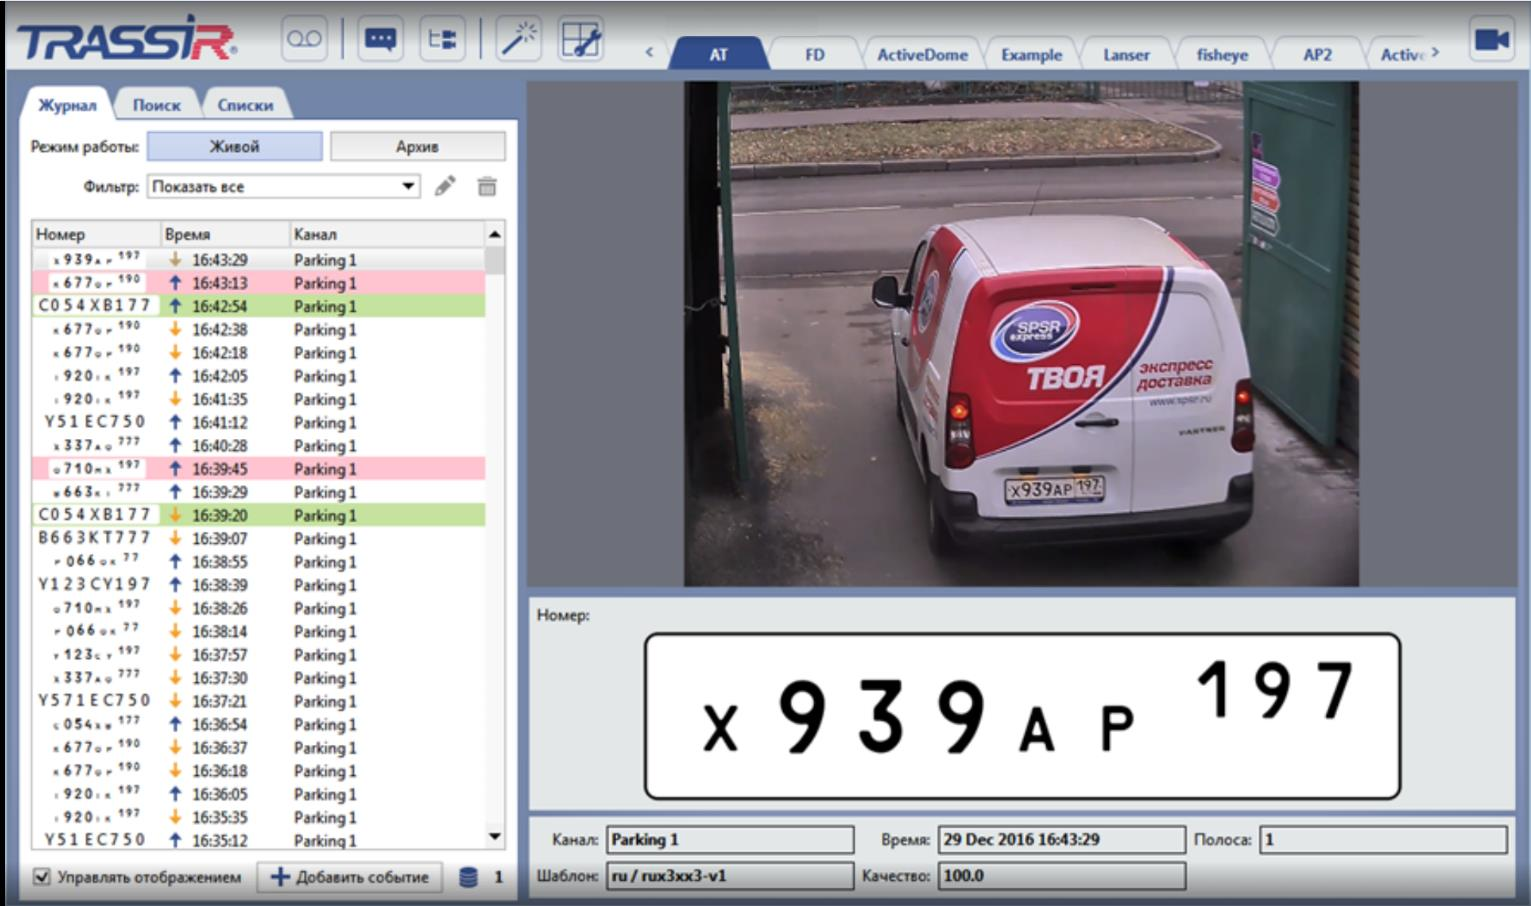
\includegraphics[width=0.4\textwidth]{trassir_example.jpg}
        \vspace{-0.8em}
        \caption{Система AutoTRASSIR 5}
    \end{figure}
\end{center}
\end{frame}

%%%%%%%%%%%%%%%%%%%%%%%%%%%%%%%%%%%%%%%%%

\begin{frame}
\frametitle{Выбор инструментов реализации}

\vspace{3em}
\begin{columns}[T,onlytextwidth]
    % Левая колонка
    \vspace{3.5em}
    \begin{column}{0.63\textwidth}
        \textbf{Инструменты в обзоре}
        \begin{itemize}
            \item Языки программирования: Python, C++
            \item Основные библиотеки: OpenCV, PIL, PyTorch
            \item Модель обнаружения: YOLO, SSD PyTorch, Detectron2
            \item Модель OCR: TesseractOCR, EasyOCR, PaddleOCR
            \item Хранилище данных: SQLite, PostgreSQL
        \end{itemize}
    \end{column}

    % Вертикальная линия
    \begin{column}{0.04\textwidth}
        \begin{center}
            \vrule width 0.5pt height 0.8\textheight
        \end{center}
    \end{column}

    % Правая колонка
    \begin{column}{0.33\textwidth}
        \textbf{Финальный выбор}
        \begin{itemize}
            \item \textbf{Python}
            \item \textbf{OpenCV} \phantom{(empty line)}
            \item \textbf{Семейство YOLO}
            \item \textbf{EasyOCR, PaddleOCR}
            \item \textbf{PostgreSQL}
        \end{itemize}
    \end{column}
\end{columns}
\end{frame}

%%%%%%%%%%%%%%%%%%%%%%%%%%%%%%%%%%%%%%%%%

\begin{frame}
\frametitle{Сбор и подготовка датасетов}

\begin{itemize}
    \item Использованы 3 датасета из открытых источников для задач сегментации автомобильных номеров
    \item Преобразованы в корректный формат для задачи детекции
    \item Итоговый датасет:
    \begin{itemize}
        \item \textbf{Тренировочная выборка}: 1 731 изображение и описание
        \item \textbf{Валидационная выборка}: 549 изображений и описаний
        \item \textbf{Тестовая выборка}: 126 изображений
        \item Всего: \textbf{2 406 изображений и 2 280 описаний}
    \end{itemize}
    \item Для оптического распознавания текста вручную составлены текстовые аннотации (2 406 аннотаций)
\end{itemize}
\end{frame}

%%%%%%%%%%%%%%%%%%%%%%%%%%%%%%%%%%%%%%%%%

\begin{frame}
\frametitle{Обучение модели детекции}

За основу для обучения на предварительных весах была взята модель YOLOv8s
\begin{itemize}
    \item Было проведено 14 обучающих итераций модели с целью нахождения оптимальных параметров
    \item Возникла проблема низкой уверенности модели на практике (0.50 - 0.60) из-за обучения с использованием оптимизатора SGD
    \item Решение было найдено путем смены оптимизатора на Adam  - уверенность модели возросла (>0.75)
\end{itemize}
\end{frame}

%%%%%%%%%%%%%%%%%%%%%%%%%%%%%%%%%%%%%%%%%

\begin{frame}
\frametitle{Реализованный прототип приложения}

При реализации приложения были достигнуты следующие результаты:
\begin{itemize}
    \item Получена высокая точность и уверенность модели распознавания
    \item Обработка одного кадра видео занимает в среднем 20 мс
    \item Реализованы распознавание текста и запись в БД без блокировки распознавания автомобильных номеров
    \item Фильтрация повторов номеров за короткий интервал 
\end{itemize}

\vspace{-1em}
\begin{figure}
    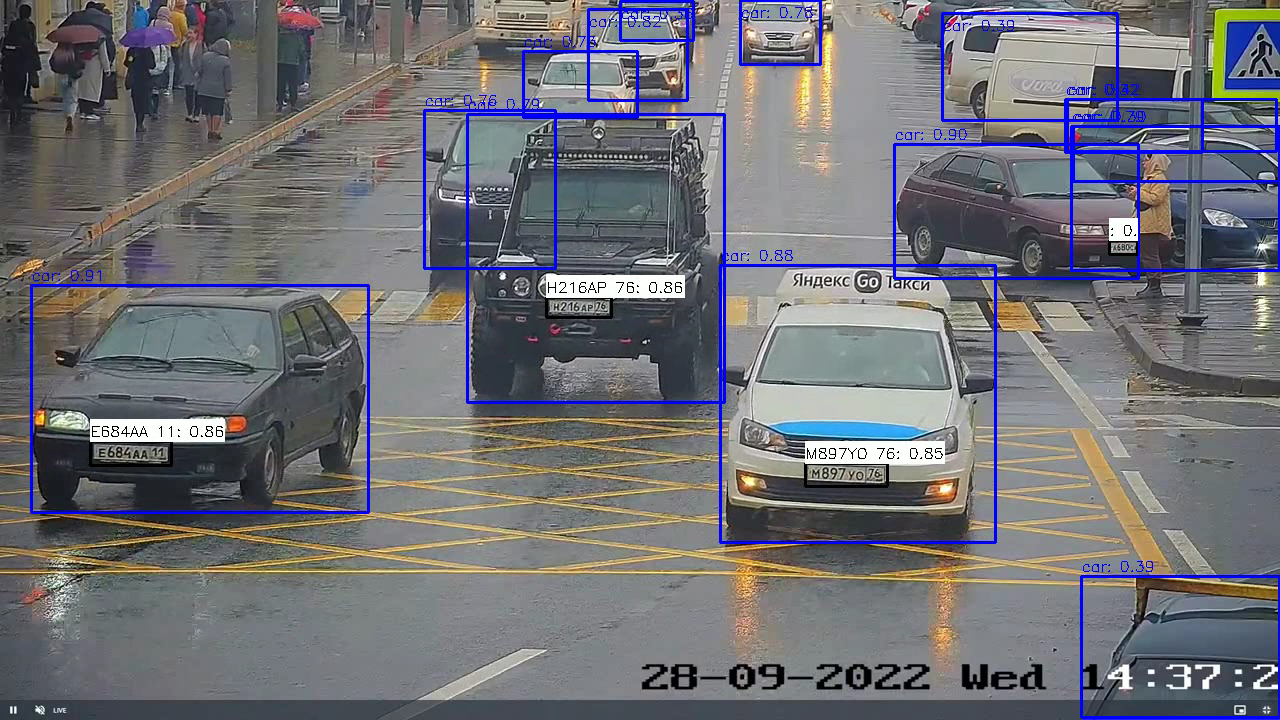
\includegraphics[width=0.6\textwidth]{detection1.png}
    \vspace{-1em}
    \caption{Демонстрация работы приложения}
\end{figure}
\end{frame}

%%%%%%%%%%%%%%%%%%%%%%%%%%%%%%%%%%%%%%%%%

\begin{frame}
\frametitle{Заключение}

В результате проделанной работы были достигнуты все поставленные задачи:
\begin{itemize}
    \item Изучены существующие технологи и решения для задачи распознавания автомобильных номеров
    \item Произведен обоснованный выбор инструментов для реализации приложения
    \item Реализован прототип приложения распознавания регистрационных знаков автомобилей
\end{itemize}

Имеются перспективы к дальнейшему развитию и улучшению приложения для практического использования в различных условиях. 

\begin{center}\bf\LARGE
Спасибо за внимание!
\end{center}

\end{frame}

\end{document}







